% !TeX spellcheck = da_DK
\documentclass[11pt,a4paper,oneside]{article}

% Overordnet opsætning
\setlength\parindent{24pt}
\setlength\parskip{3pt}
\setlength{\headheight}{14pt}
\renewcommand{\baselinestretch}{1.7}

\usepackage[utf8]{inputenc}
\usepackage[danish,english]{babel}
\usepackage{amsfonts,amsmath} %math: align og gather mm.; fonts: flere forskellige symboler
\usepackage[left=2cm, right=2cm, bottom=2cm]{geometry}
\usepackage{enumitem} %anvendes til ændring i itemize mm.
\usepackage{fancyhdr} %Opsaening af sidehoved og -fod
\usepackage{lastpage} % Side "x af X".
\usepackage[ocgcolorlinks,linkcolor=black]{hyperref}
\usepackage{indentfirst} %"Indent" efter section og chapters etc.
\usepackage{graphicx} % for plotting graphs in matrix
\usepackage{subcaption} % figure "footnotes"
\usepackage[font=small,compatibility=false]{caption}
\usepackage[nottoc,numbib]{tocbibind}    
\usepackage{ mathrsfs }
\usepackage{bbold}
\usepackage{setspace}



% bibliography
\usepackage{csquotes}
\usepackage{biblatex}
\addbibresource{bibliography.bib}

% Ændring af titler
\usepackage{sectsty}
\subsectionfont{\normalfont\bfseries}
\subsubsectionfont{\itshape}

%Rstudio pakker
\usepackage[svgnames]{xcolor}
\usepackage{listings}

\lstset{language=R,
basicstyle=\scriptsize\ttfamily,
commentstyle=\ttfamily\color{gray},
numbers=left,
numberstyle=\ttfamily\color{gray}\footnotesize,
stepnumber=1,
numbersep=5pt,
backgroundcolor=\color{white},
showspaces=false,
showstringspaces=false,
showtabs=false,
frame=single,
tabsize=2,
captionpos=b,
breaklines=true,
breakatwhitespace=false,
title=\lstname,
escapeinside={},
keywordstyle={},
morekeywords={}
}

% fancy table
\usepackage{booktabs}
\usepackage{multirow}
\pagestyle{fancy}
\fancyhf{}
\fancyhead[L]{\leftmark}
\fancyhead[R]{\rightmark}
\lfoot{\author}
\rfoot{\thepage}
\renewcommand{\headrulewidth}{0.4pt}
\renewcommand{\footrulewidth}{0.4pt}

%symbolforkortelser
\newcommand{\lll}{\mathcal{L}}
\newcommand{\LL}{\Leftrightarrow}
\newcommand{\lp}{\left(}
\newcommand{\rp}{\right)}
\newcommand{\rb}{\right]}
\newcommand{\lb}{\left[}
\newcommand{\lc}{\left\{}
\newcommand{\rc}{\right\}}
\newcommand{\dd}{\mathrm{d}}
\newcommand{\cc}{\mathbb{C}}
\newcommand{\aaa}{\mathbf{A}}
\newcommand{\ee}{\mathbf{E}}
\newcommand{\ff}{\mathcal{F}}
\newcommand{\ggg}{\mathcal{G}}
\newcommand{\hh}{\mathcal{H}}
\newcommand{\pp}{\mathcal{P}}
\newcommand{\qq}{\mathcal{Q}}
\newcommand{\vv}{\mathbf{V}}
\newcommand{\rr}{\mathbf{R}}
\newcommand{\nn}{\mathbf{N}}
\newcommand{\zz}{\mathbf{Z}}
\newcommand{\yy}{\mathbf{Y}}
\newcommand{\nnn}{\mathcal{N}}
\newcommand{\ii}{\mathbf{1}}
\newcommand{\bs}{\text{BS}}
\newcommand{\sumn}{\sum_{i=1}^n}
\renewcommand{\theequation}{1.\arabic{equation}}
\DeclareMathOperator*{\argmin}{\arg\,\min}
\newcommand{\RNum}[1]{\uppercase\expandafter{\romannumeral #1\relax}}

\selectlanguage{english}

\lstset{language=R}

% Environment for theorems etc.
\newtheorem{theorem}{Theorem}[section]
\newtheorem{corollary}{Corollary}[theorem]
\newtheorem{lemma}[theorem]{Lemma}
\newtheorem{assumption}{Assumption}
\newtheorem{proof}{Proof}
\newtheorem{mydef}{Definition}

% Colour citation links (otherwise they are luminescent green)
\hypersetup{colorlinks,linkcolor={black},citecolor={black},urlcolor={black}} 

% TOC depth
\setcounter{tocdepth}{2}

\title{Data}
\author{William Gram \& Kristian Strand}
\date{\today}

\begin{document}

\pagenumbering{gobble}
\maketitle

\newpage

\pagenumbering{roman}
\rfoot{\thepage}

\tableofcontents

\newpage

\pagenumbering{arabic}
\setcounter{page}{1}

\section{Data}
\subsection{Data introduction}
\noindent In the following section we will describe the data used to fit our HMM model. The goal is to achieve a data set which reflects the full investment universe for institutional as well as retail investors. As we are restricted in terms of data availability, we choose to focus on U.S. return data only. Our analysis can easily be extended to reflect a more global investment universe if one have access to global return data on various asset classes.   

One of our contributions to the existing literature on HMM and asset allocation, is the inclusion of a more granular investment universe. For example Guidolin \& Timmermann (2007) \cite{2007} uses only three different asset classes ("large stocks", "small stocks" and 10-year T-bonds). Splitting up major asset classes will offer investors a broader palette of risk-reward profiles. This concept is developed in classic Markowitz portfolio theory (MPT) first seen in Markowitz (1952)\cite{MPT52}. The inclusion of more asset classes provides investors with broader diversification opportunities. We will work with two different bond indices, namely high yield bonds (HY) and investment grade bonds (IG), both of which are corporate bond indices with inherently different risk levels. In addition, we will use one commodity index (CI), a small cap stock index given by Russell 2000 (R2000) and a large cap stock index given by Russell 1000 (R1000). Figure \ref{riskreward} below presents a scatter plot of these different asset classes. Returns in figure \ref{riskreward} are all in excess of the risk free return.  

MPT states that higher returns cannot generally be achieved without simultaneously increasing risk as measured by standard deviation often referred to as volatility. From figure \ref{riskreward} it is apparent that the different asset classes provide different risk-reward trade-offs with a trend toward higher volatility for higher return. In isolation, investing in R1000 brings higher return than investing in R2000. This is exacerbated when considering return per unit of volatility. The figure does not, however, illustrate the benefits of diversification, as advocated in MPT. This motivates the inclusion of assets which may in isolation have poor risk-reward profiles. We will define the risk-reward profile of an asset class through its Sharpe ratio (SR), the ratio of excess returns to volatility. 

In the following we will provide a description of the asset classes that we are considering. Following that we will describe these asset classes by standard statistical properties. All data is collected from Bloomberg and the period in consideration is July 31 1983 to December 31 2018.    


\begin{figure}[ht]
\centering
\vspace{4mm}
\caption{Risk reward profiles for US asset classes}
\label{riskreward}
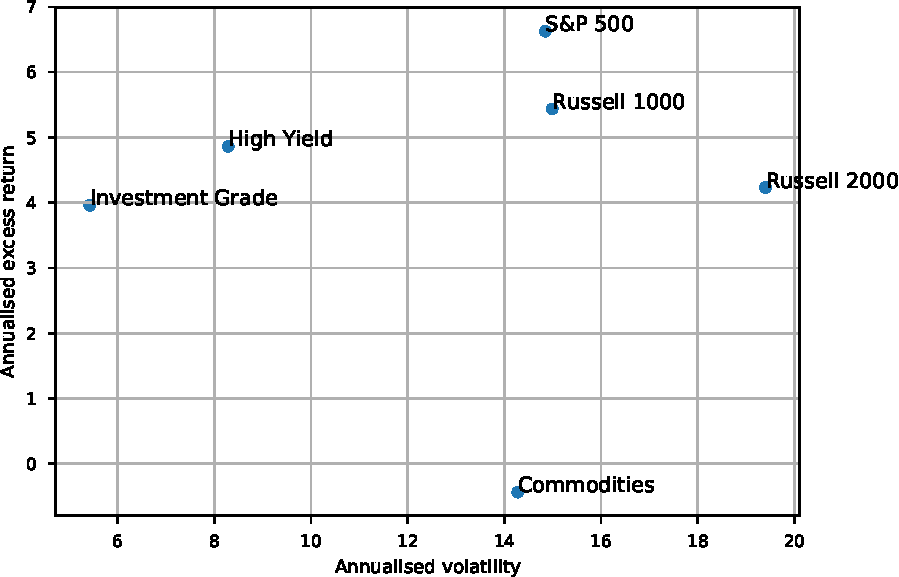
\includegraphics[scale=1]{images/Sharpes.pdf}
\begingroup
\vspace{4mm}
\subcaption*{\textit{For data description we refer to section \ref{datadescription} and for definitions of returns we refer to section \ref{descriptivesection}}}
\endgroup
\end{figure}



\subsection{Data description}\label{datadescription}

\subsection*{Investment Grade Bond Index}
\noindent We will work with the " Bloomberg Barclays US Credit Total Return Index (LUACRTRUU:IND)", which we will refer to as the "IG index". The index is an unhedged \$-index. IG bonds are rated Baa3/BBB-/BBB- or higher using the middle rating of Moody's, S\&P and Fitch. The US corporate IG market is currently around \$5 trillion. With a total US corporate credit market of roughly \$7.5 trillions this amounts to 68\% of the total US corporate credit market\cite{Bloomberg}. In the next section in table \ref{returnstats} we present historical excess log-return statistics for each asset class.

\subsection*{High-Yield Bond Index}
\noindent In contrast to the relatively low-risk IG space, we will work with the "Bloomberg Barclays US Corporate High Yield Total Return Index (LF98TRUU:IND)", which we will refer to as the "HY index". The index is an unhedged \$-index, comprised of HY bonds denominated in \$ with a mininum size of \$150mn. The index dates back to july 1983 for monthly data and to august 1998 with daily data. HY bonds are corporate bonds, which middle rating of Moody's, Fitch and S\&P, is Ba1/BB+/BB+ or below. Pre the 80's HY bonds were bonds of outstanding fallen angles. i.e former investment grade companies that had been downgraded. Today HY bonds are often used to finance strategic mergers and acquisitions or  by leveraged-buy-out firms to provide means of capital for highly leveraged companies. From 1998 to 2018 the US HY bond market expanded almost six fold\cite{Pimpco}. According to Bloomberg the current total size of the US corporate debt market is \$7.5 trillion of which 16.1\% (\$1.21 trillion) are HY bonds. Leveraged Loans represent roughly the same as high yield bonds, while the remaining 68\% are investment grade bonds\cite{Bloomberg}. We have chosen not to include leveraged loans in our analysis. We are aware that leveraged loans and HY bonds are not perfect substitutes for an investor, however we believe that they are similar enough to not affect conclusions substantially.         

\subsection*{Russell 1000 and Russell 2000}
\noindent To reflect that large cap stocks and small cap stocks offers two different investment opportunities, we will work with two stock indices, namely Russell 1000 and Russel 2000, which are both subsets of the broader Russell 3000. Russel 3000 is a broad U.S stock index and represents approximately 98\% of the U.S. public equity market.     

Russell 1000 is a U.S. large-cap stock index  composed of approximately 1,000 of the largest U.S. companies. It represents roughly 90\% of the total market capitalisation of all listed U.S. stocks and is considered one of the leading large cap indicators on equal footing with S\&P500 and NASDAQ Composite. We will work with the "Russell 1000 Total Return (INDEXRUSSELL:RUITR)", which assumes dividends are reinvested. Russel 2000 is a U.S. small-cap stock index. The index represents 8\% of the public U.S. sotkc market and serves as a benchmark for U.S. small-cap stocks. As with Russell 1000 we will use the total return index, namely "Russell 2000 Total Return (INDEXRUSSELL:RUTTR)". 

\subsection*{Commodities}
\noindent We will make use of the "Bloomberg Commodity Index Total Return Index (BCOMTR:IND)", which we will refer to as the "commodity index". The index is made up of 22 exchange-traded futures on 20 physical commodities. It is weighted to account for economic significance and market liquidity. As per december 2018 crude brent oil and gold represent 8.5\% and 11.57\%, respectively. 

\subsection*{Risk free rate}
\noindent In choosing the risk free rate  we follow common practice in academia and use the yield on short term government bills\cite{riskfreerate}. Specifically we will follow Fama and French and use the 1-Month TBill rate from Ibbotson and Associates Inc, which is provided from Kenneth French's database. 

\subsection{Descriptive statistics}\label{descriptivesection}
\noindent In this section we consider the empirical moments of our asset classes. We will not assume any data generating processes for the asset class returns. Consequently, we are not suggesting that the empirical estimates are expressions for the population moments. We will define the empirical moments in the following way.
\vspace{-7mm}
\begin{gather}
    r_{t,a}=(\ln{p_{t,a}}-\ln{p_{t-1,a}})\cdot 100
    \\
    \hat{\Bar{r}}_a=\frac{1}{T}\sum_{t=1}^{T}r_{t,a}, \qquad \hat{\sigma}= \sqrt{\frac{1}{T}\sum_{t=1}^{T}(r_{t,a}-\hat{\Bar{r}}_a)^2} \label{meanvol} \\ 
    \widehat{\text{skew}}_a=\frac{\frac{1}{T}\sum_{t=1}^{T}(r_{t,a}-\hat{\Bar{r}}_a)^3}{\lb\frac{1}{T}\sum_{t=1}^{T}(r_{t,a}-\hat{\Bar{r}}_a)^2\rb^{3/2}}
    , \qquad \widehat{\text{kurt}}_a=\frac{\frac{1}{T}\sum_{t=1}^{T}(r_{t,a}-\hat{\Bar{r}}_a)^4}{\lb\frac{1}{T}\sum_{t=1}^{T}(r_{t,a}-\hat{\Bar{r}}_a)^2\rb^{2}} \label{skewkurt},
\end{gather}
where $a \in \{1,2,...,A\}$ denotes asset class a. Additionally, we will consider the auto correlation function (ACF) to shed light on time dependency in the return processes. We will consider two ACFs, namely that of returns and that of absolute returns. The advantage of considering the ACF for absolute returns rather than squared returns is, that it only requires existence of fourth order moments rather than eight order moments (find kilde på dette vedrører sandsynligvis Hölders teorem). The two ACFs are defined as:
\begin{align}
    \text{ACF}_a(h,r_t)&= \frac{\frac{1}{T}\sum_{t=1}^{T}(r_{t,a}-\hat{\Bar{r}})(r_{t-h,a}-\hat{\Bar{r}})}{\sqrt{\frac{1}{T}\sum_{t=1}^{T}(r_{t,a}-\hat{\Bar{r}})^2}\sqrt{\frac{1}{T}\sum_{t=1}^{T}(r_{t-h,a}-\hat{\Bar{r}})^2}} \label{acf} ,  \\
    \text{ACF}_a(h,\vert {r_t} \vert) &= \frac{\frac{1}{T}\sum_{t=1}^{T}(\vert r_{t,a} \vert-\vert\hat{\Bar{r}}\vert)(\vert r_{t-h,a}\vert-\vert\hat{\Bar{r}}\vert)}{\sqrt{\frac{1}{T}\sum_{t=1}^{T}(\vert r_{t,a}\vert-\vert\hat{\Bar{r}}\vert)^2}\sqrt{\frac{1}{T}\sum_{t=1}^{T}(\vert r_{t-h,a}\vert-\vert\hat{\Bar{r}}\vert)^2}} \label{acfabs}. 
\end{align}

\noindent Applying the moment estimates as defined in equation (\ref{meanvol})-(\ref{skewkurt}) to the monthly excess returns we generate table \ref{descriptive_statistics}. Monthly excess mean returns span from -0.04\% for the commodity index to 0.55\% for S\&P500. The monthly standard deviation spans between 1.6\% for the IG index to 5.6\% for Russell 2000. All asset classes exhibit negative skewness in returns while the excess kurtosis indicates heavy tails of the return distribution. These findings are in line with literature in financial time series e.g. Taylor (2011)\cite{Taylor}.           

\begin{table}[h!]
\centering
\captionsetup{justification=centering,margin=0.6cm}
\caption{Descriptive summary of monthly excess returns}
\label{descriptive_statistics}
\begin{tabular}{lrrrrrr}
\toprule
{} &    mean &     std &  ann. mean &  ann. std &  kurtosis &  skewness \\
\midrule
High Yield       &  0.4052 &  2.3925 &     4.8619 &    8.2879 &   10.1555 &   -1.1786 \\
Investment Grade &  0.3297 &  1.5647 &     3.9570 &    5.4204 &    3.4863 &   -0.4526 \\
Commodities      & -0.0363 &  4.1218 &    -0.4357 &   14.2782 &    3.0823 &   -0.5984 \\
Russell 2000     &  0.3526 &  5.6021 &     4.2314 &   19.4063 &    5.4437 &   -1.2441 \\
Russell 1000     &  0.4531 &  4.3279 &     5.4368 &   14.9922 &    3.9511 &   -1.0928 \\
S\&P 500          &  0.5522 &  4.2869 &     6.6258 &   14.8501 &    3.8178 &   -1.0510 \\
Risk Free        &  0.2931 &  0.2324 &     3.5167 &    0.8050 &   -0.8818 &    0.3011 \\
\bottomrule
\end{tabular}
\caption*{Source: Bloomberg and Kenneth French data base.
Period: Aug. 31 1983 to Dec. 31 2018. \\ Kurtosis is excess of that of the normal distribution}
\end{table}

\noindent Figure \ref{index_levels} presents each asset class indexed with July 31 1983=100



   









\clearpage

\begin{figure}[ht]
\center
\caption{Index values for US asset classes 1983-2018}
\vspace{-0mm}
\label{index_levels}
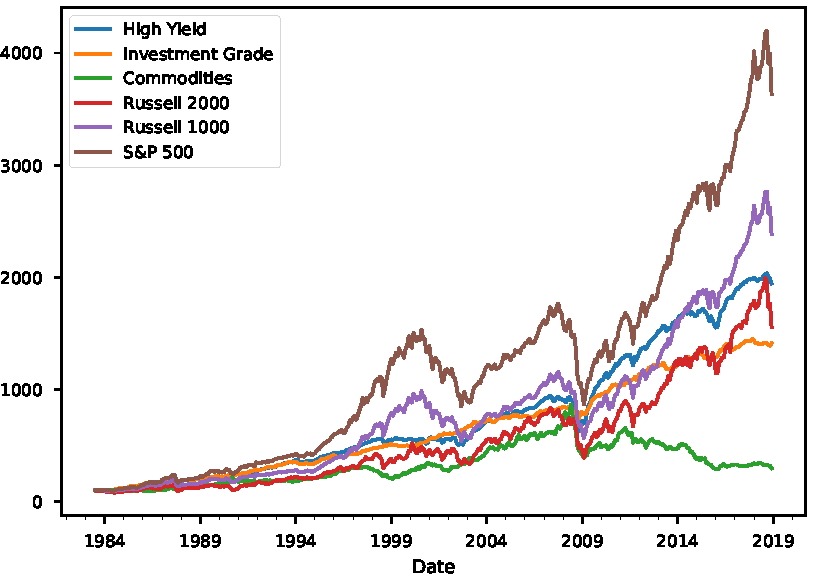
\includegraphics[scale=1]{images/Prices.pdf}
\begingroup
\subcaption*{\textit{Source: Bloomberg}}
\endgroup
\end{figure}


\clearpage

\begin{figure}[p]
    \caption{Monthly excess returns}
    \makebox[\linewidth]{
        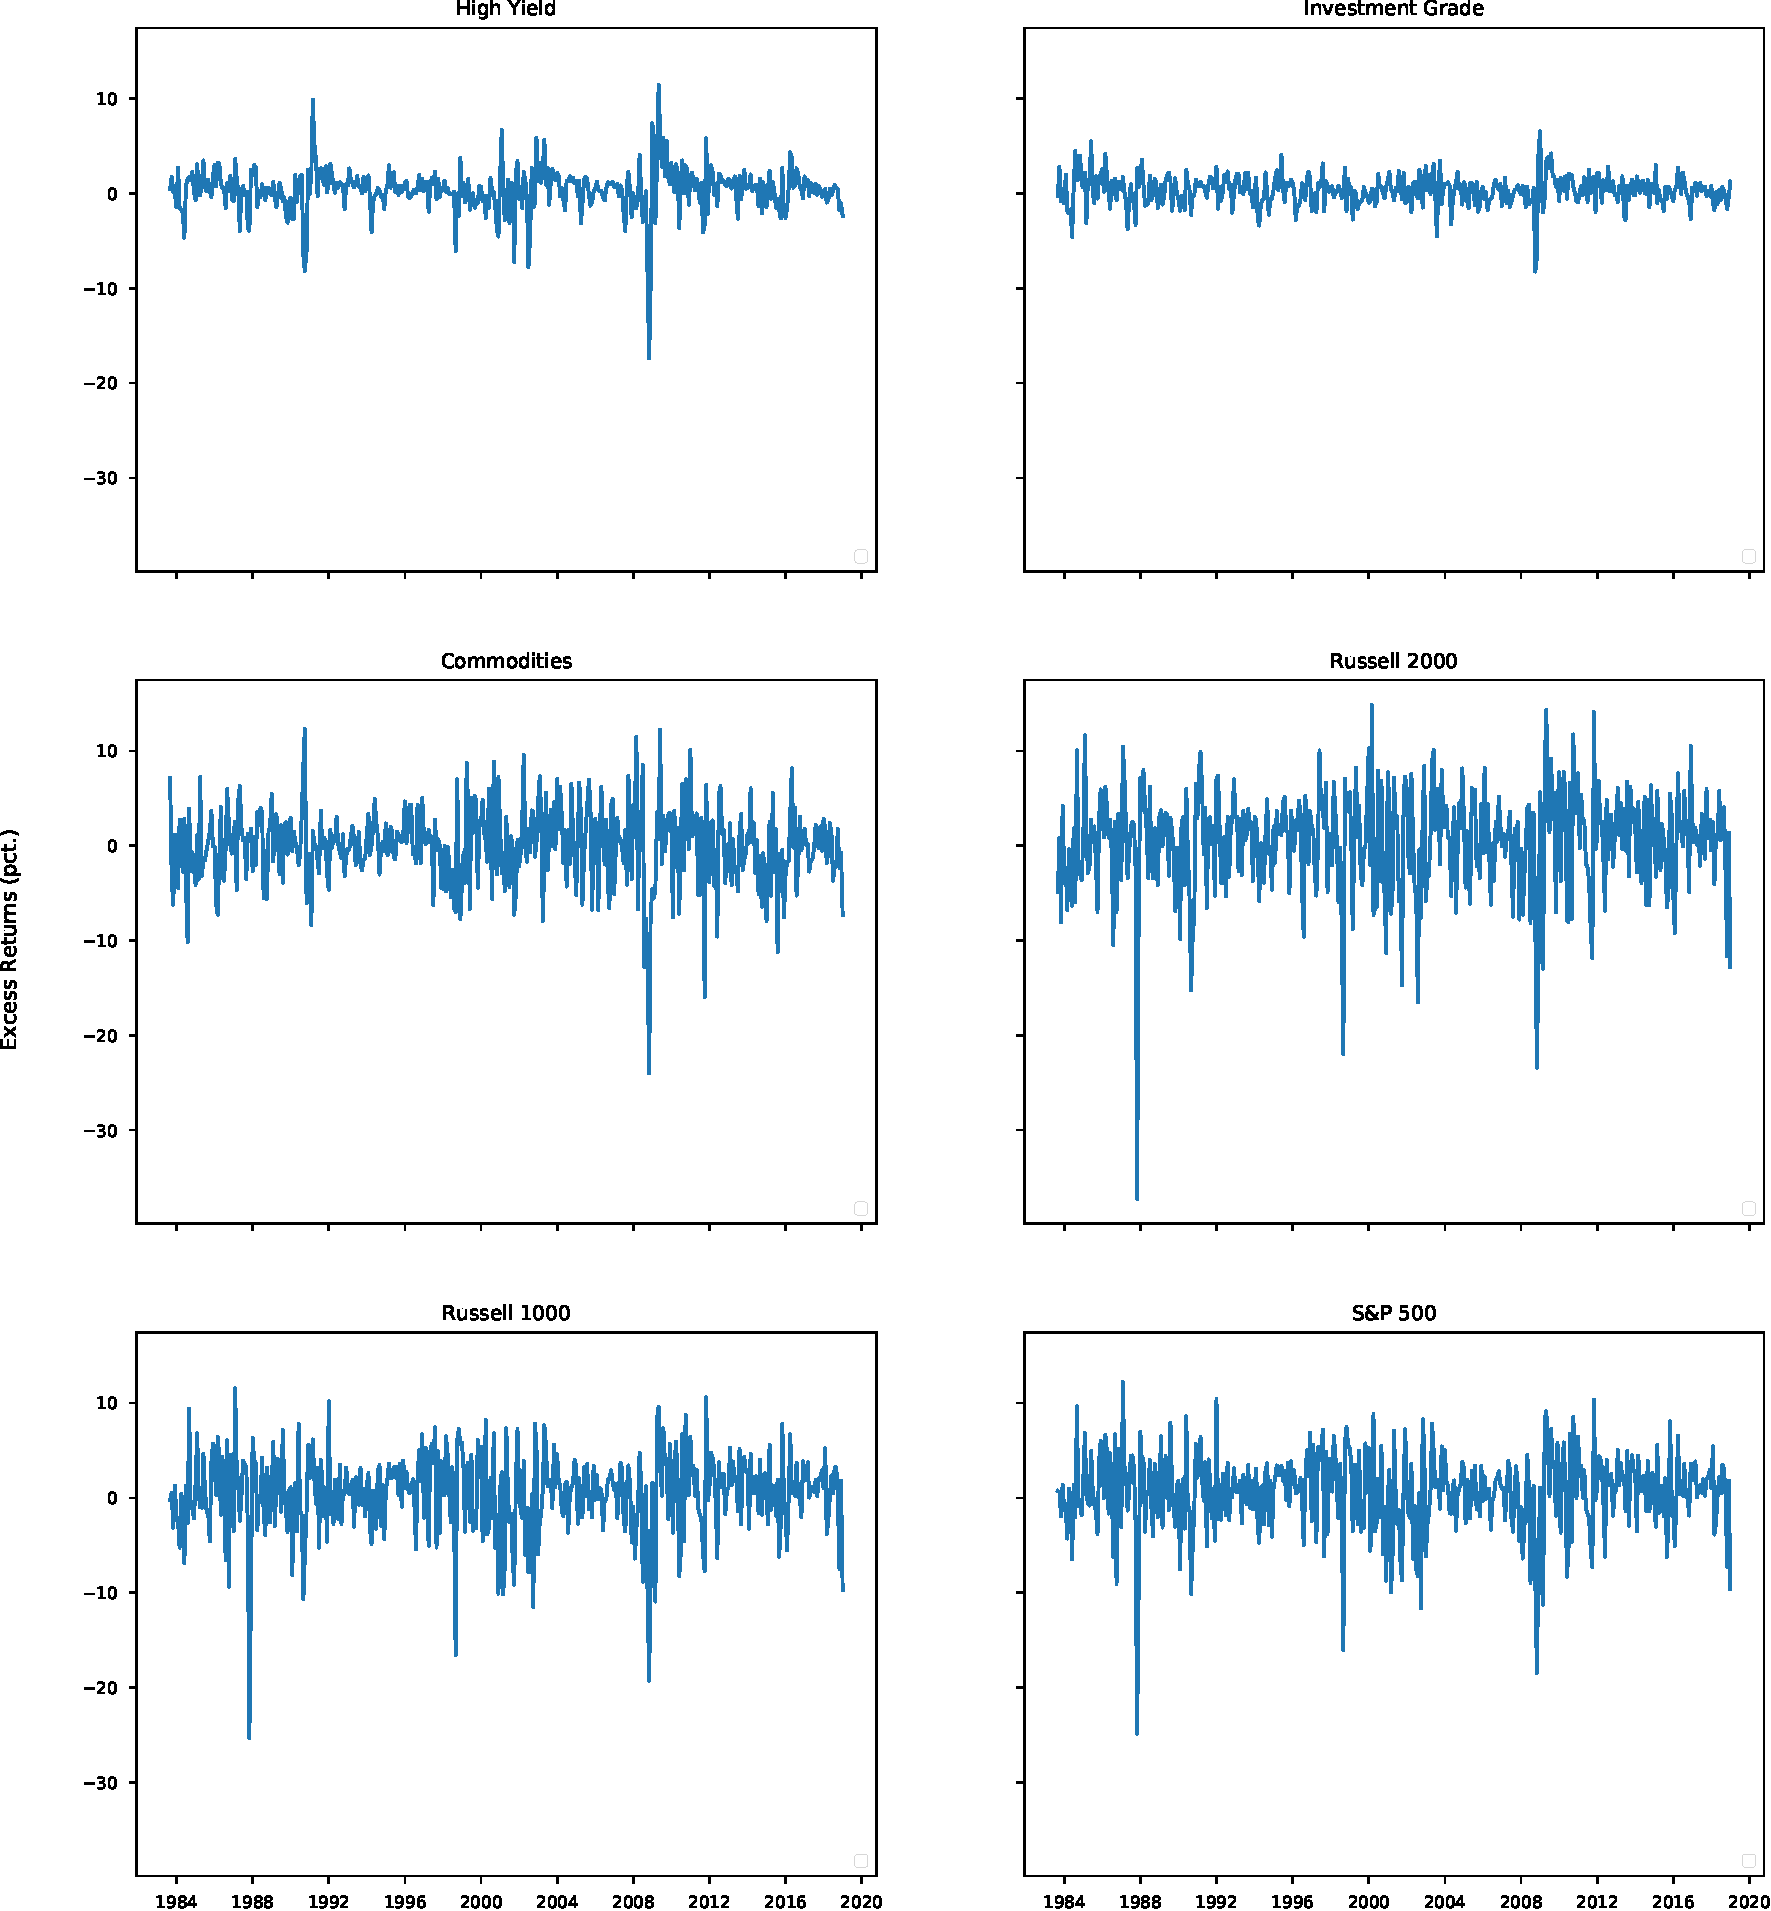
\includegraphics[width=1\linewidth, height=0.85\textheight]{images/ExcessReturns.pdf}
    }
\end{figure}

\clearpage


\noindent The graphical inspection in figure \ref{mth_returns}-\ref{autocorr} shows that all returns, to some extent, exhibit volatility clustering. That is especially clear around the peak of the financial crisis in 2008-09 and for most asset classes also in the mid-late 1980's probably explained by "black Monday in 1987" and "black Friday in 1989". Furthermore, a graphical comparison of returns to their corresponding normal distributions indicates that returns are non-normal and are negatively skewed with fat tails. The (linear) auto correlation functions of returns indicates very little to no auto correlation at all. The conclusion to the graphical inspection is that the data exhibit the stylised facts for financial data, i.e. heavy tails, absence of auto correlation but with non-linear dependencies (among others through the second moment)\cite{Cont}.  





\subsection{Normality test and the need for more sophisticated models}
\noindent It is a well known stylised fact that financial data is non-normal and the informal inspection in the previous section pointed towards the same conclusion. To formally test for normality in the data generating process of asset returns, we will use D’Agostino-Pearson test.    


  
\clearpage  
  


\clearpage

\begin{figure}[ht]
\center
\caption{Monthly returns from 1983-2018}
\vspace{-0mm}
\label{mth_returns}
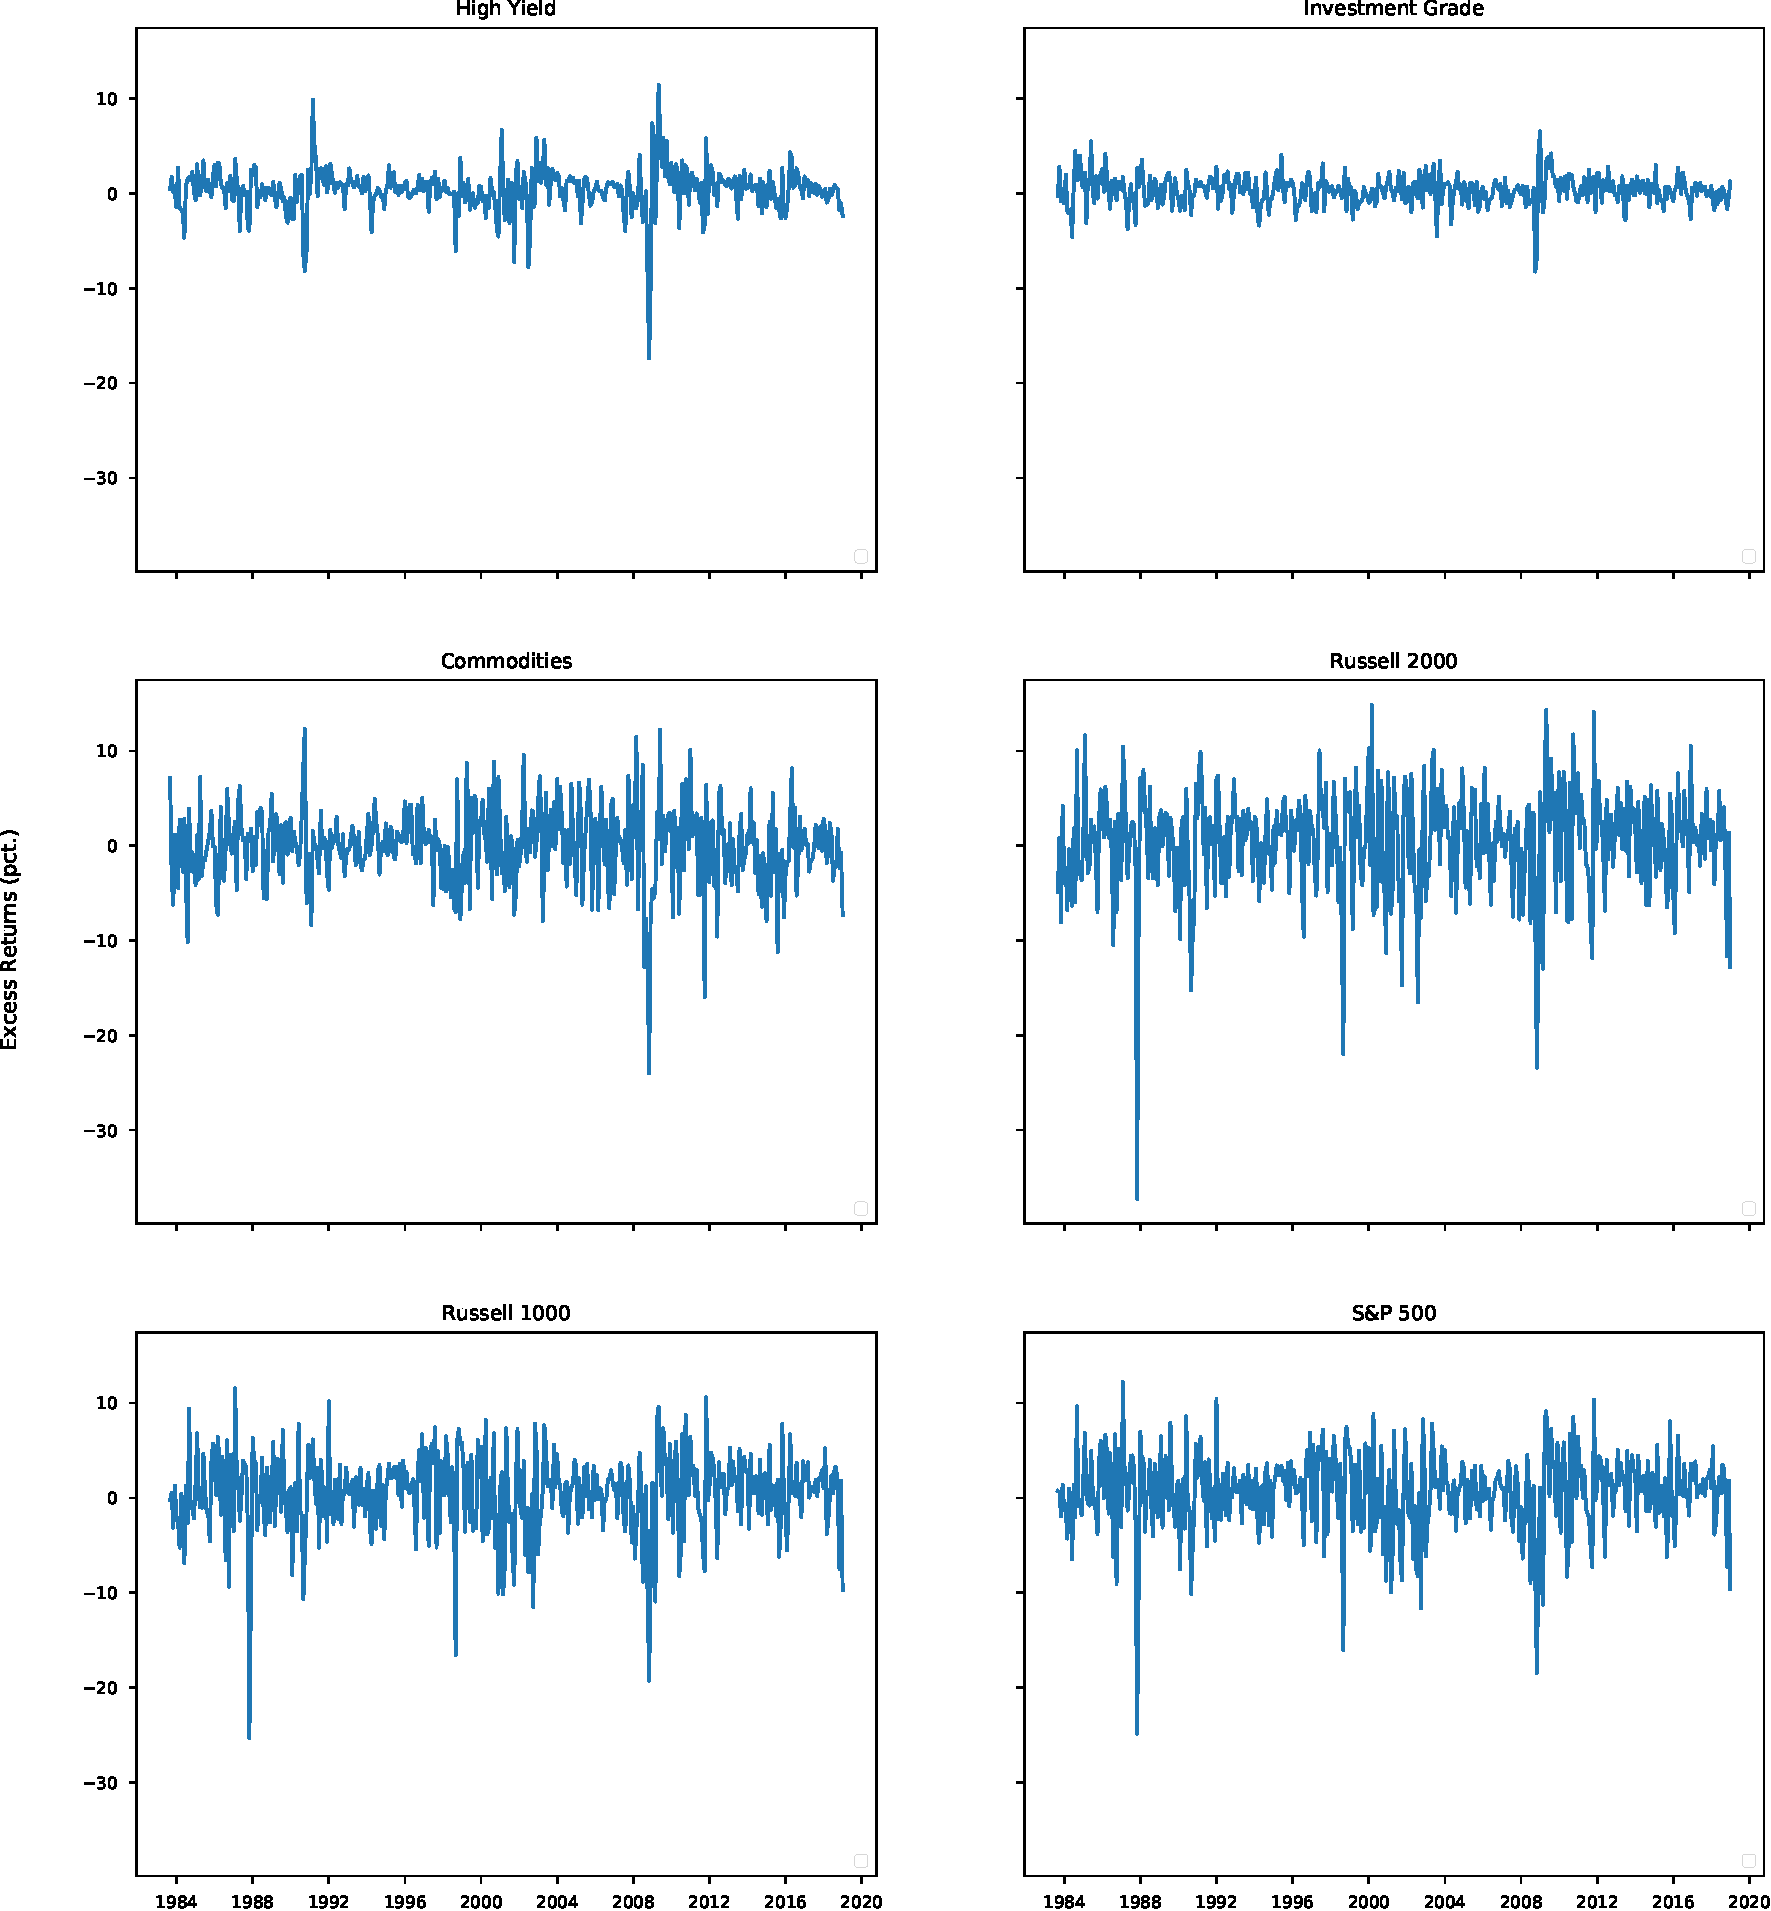
\includegraphics[width=\textwidth,height=\textheight,keepaspectratio]{images/ExcessReturns.pdf}
\begingroup
\vspace{-14mm}
\subcaption*{\textit{Source: Bloomberg and own calculations}}
\endgroup
\end{figure}

\clearpage

\begin{figure}[ht]
\center
\caption{Monthly volatility from 1983-2018}
\vspace{-0mm}
\label{mth_vol}
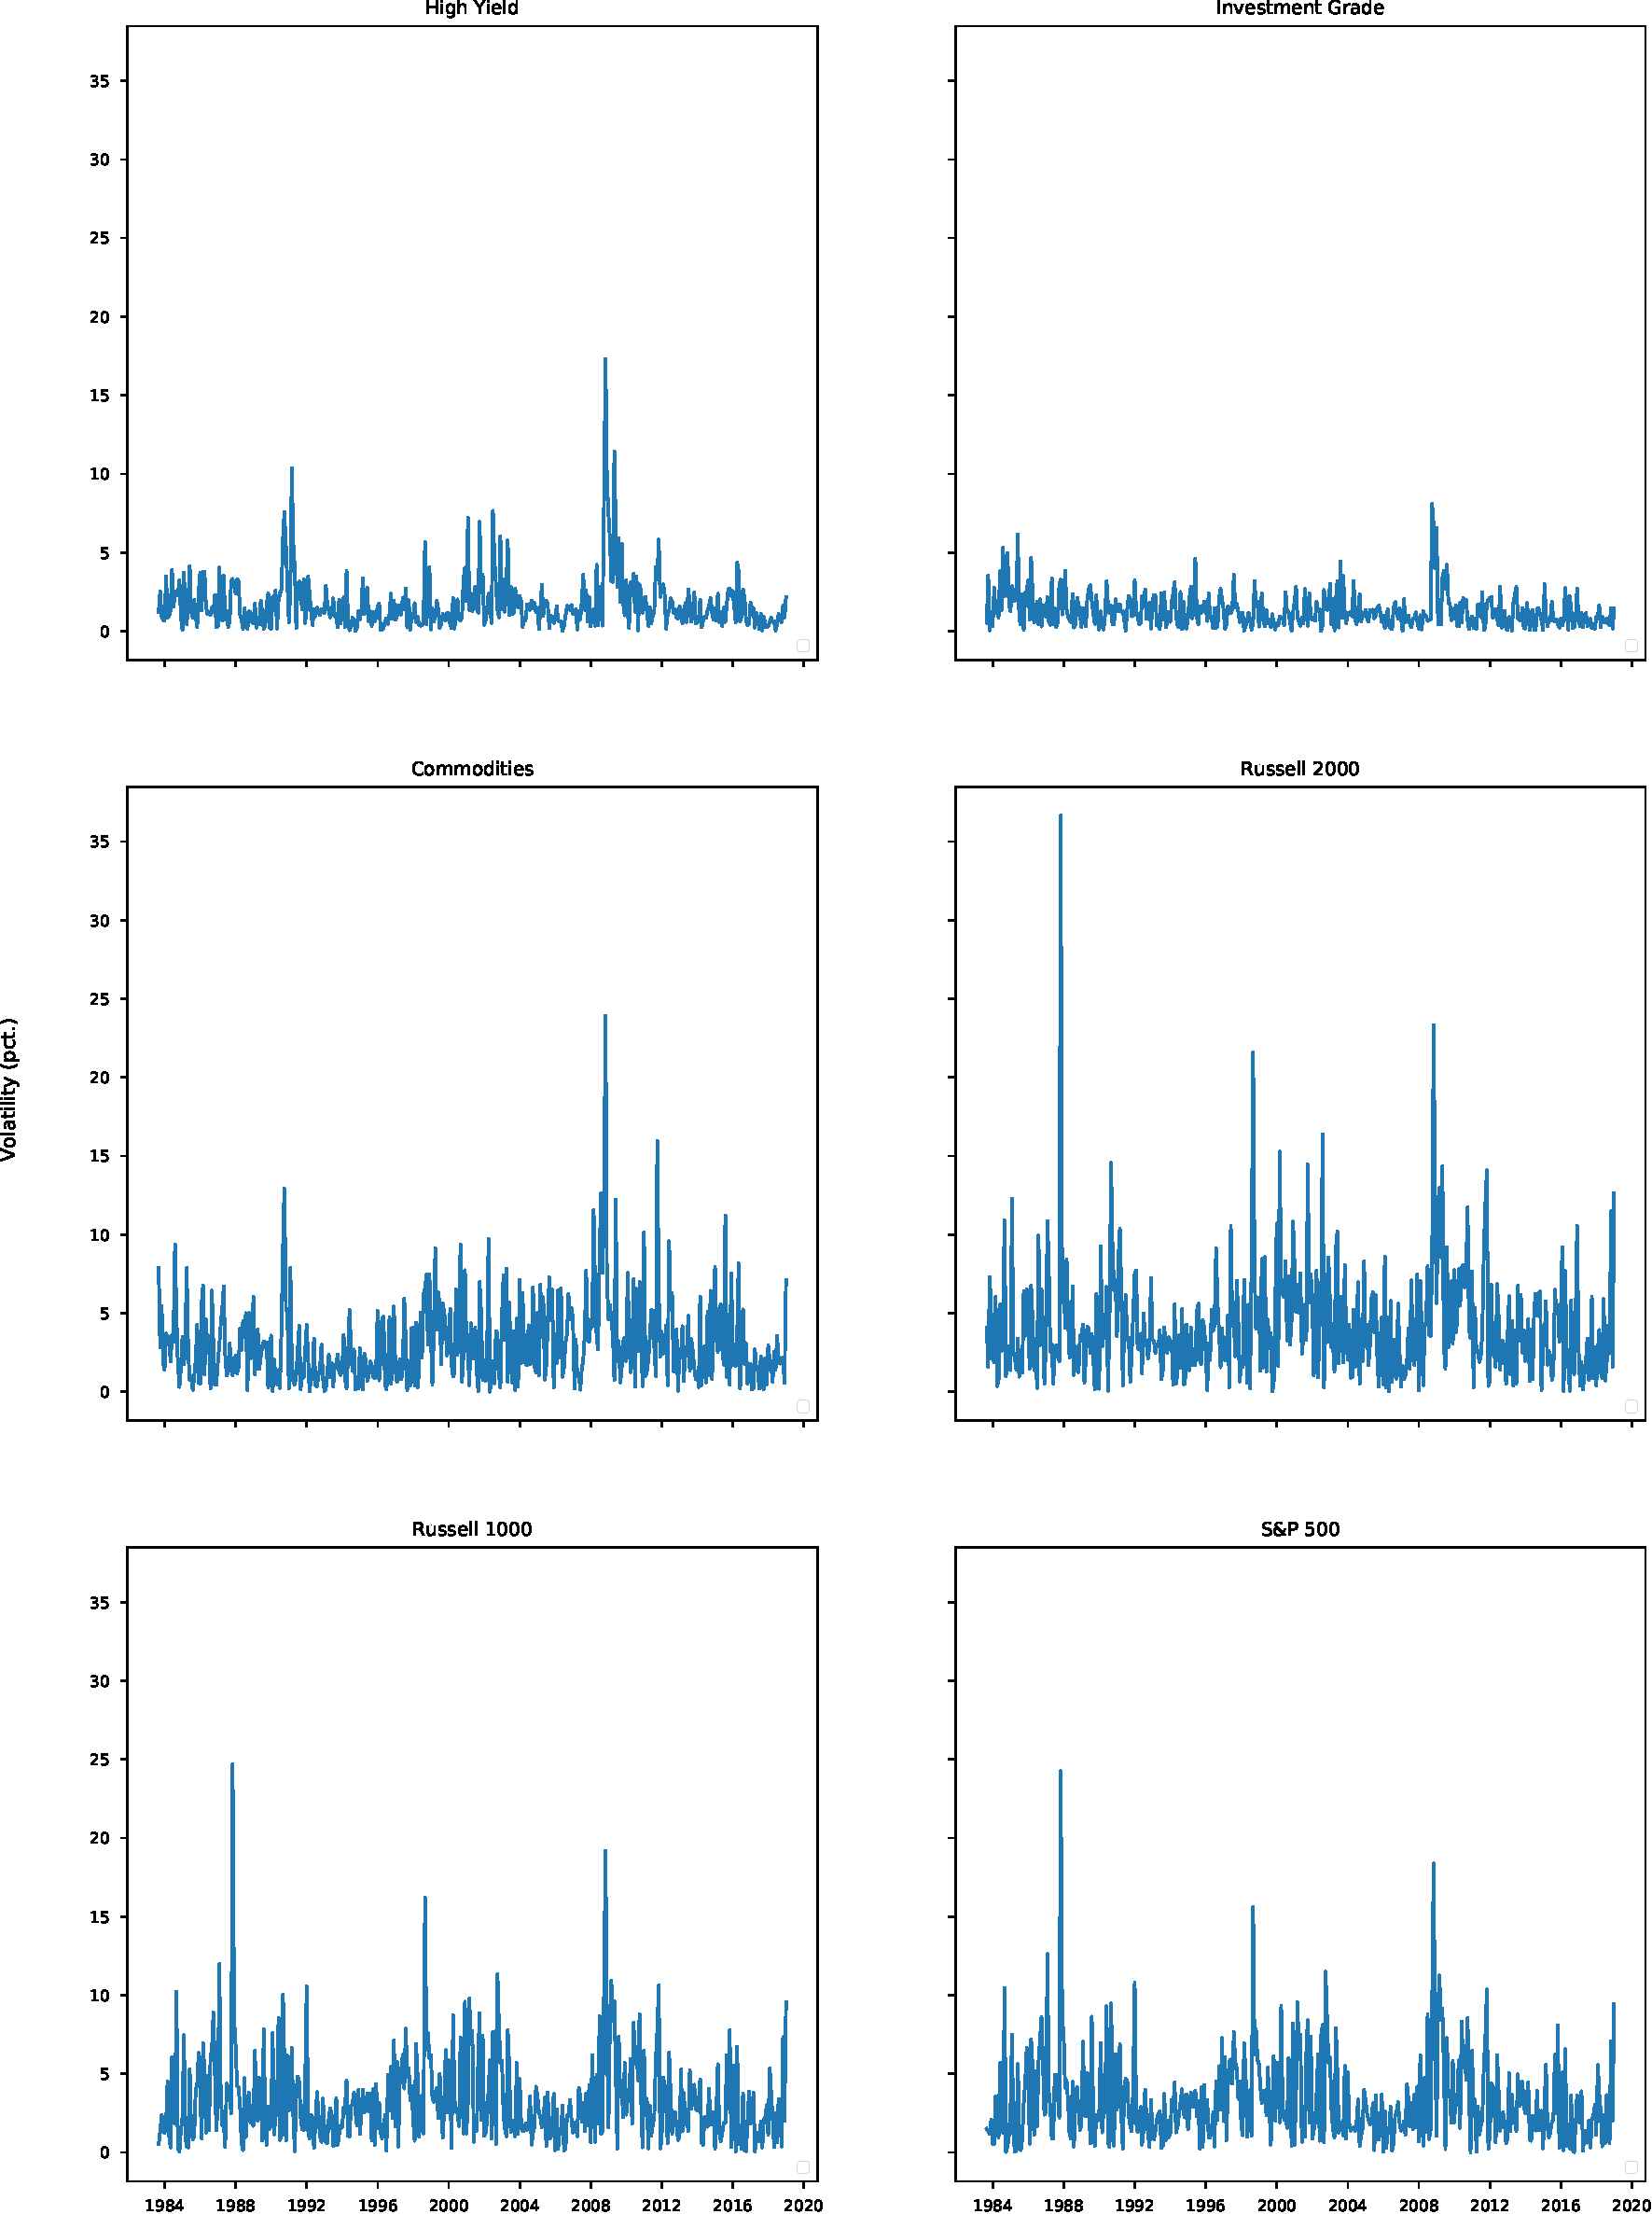
\includegraphics[width=\textwidth,height=\textheight,keepaspectratio]{images/Vol.png}
\begingroup
\vspace{-14mm}
\subcaption*{\textit{Source: Bloomberg and own calculations}}
\endgroup
\end{figure}

\clearpage

\begin{figure}[ht]
\center
\caption{Distribution of monthly returns from 1983-2018}
\vspace{-0mm}
\label{returns_dist}
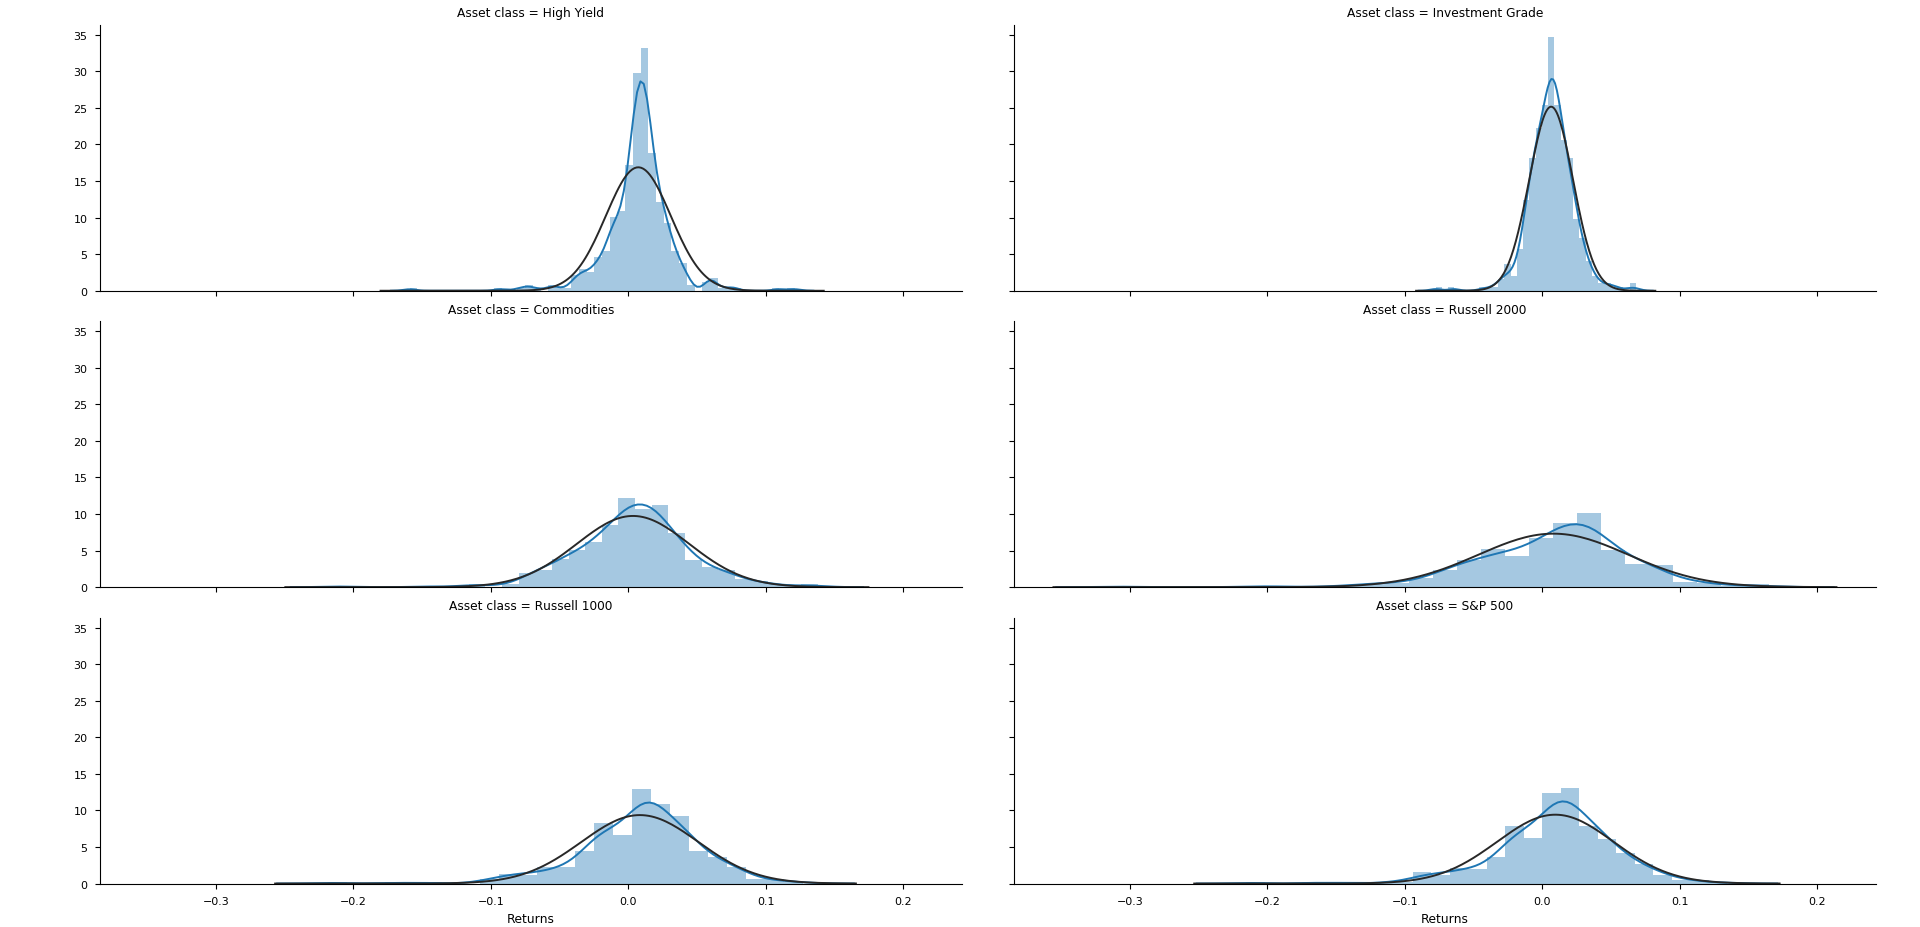
\includegraphics[width=\textwidth,height=500pt]{images/return_distributions.png}
\begingroup
\vspace{-14mm}
\subcaption*{\textit{Source: Bloomberg and own calculations}}
\endgroup
\end{figure}

\clearpage


\begin{figure}[ht]
\center
\caption{Autocorrelation functions}
\vspace{-0mm}
\label{autocorr}
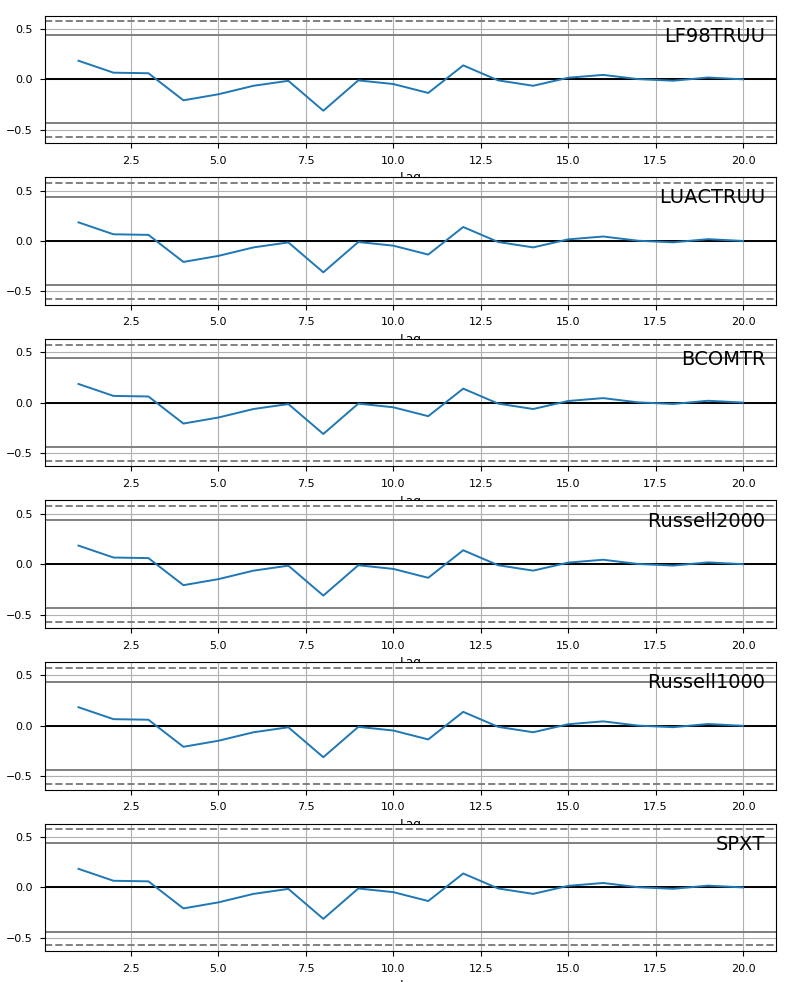
\includegraphics[width=\textwidth,height=\textheight,keepaspectratio]{images/autocorr_fct.png}
\begingroup
\vspace{-5mm}
\subcaption*{\textit{Source: Bloomberg and own calculations}}
\endgroup
\end{figure}



\clearpage





   
%We consider US return data for several asset classes, which reflects a large part of the potential investment universe for both institutional and retail investors.   

%https://intelligent.schwab.com/public/intelligent/insights/whitepapers/asset-allocation.html

\printbibliography[heading=none]

\end{document}